\documentclass[11pt]{article}
\usepackage[margin=1in]{geometry}
\usepackage{amsmath,amssymb}
\usepackage{graphicx}
\usepackage{booktabs}
\usepackage[colorlinks=true,linkcolor=blue,citecolor=blue,urlcolor=blue]{hyperref}

% --- the only two lines to edit before submission ---
\newcommand{\authorname}{Singularity}
\newcommand{\affiliation}{}

\title{When does a test pay off at dry-off?\\ Decision curve analysis for selective dry-cow therapy}
\author{\authorname\\ \small \affiliation}
\date{\today}

\begin{document}
\maketitle

\begin{abstract}
Selective dry-cow therapy gives antibiotics at dry-off only to cows that a test flags as infected, and an internal
teat sealant to all. Evaluations so far use sensitivity and specificity, or partial budgets in currency. Neither
answers the question a veterinarian faces: \emph{for my herd and my view of the trade-off between antibiotic use and
missed infections, is the test better than treating every cow, or none?} Decision curve analysis, standard for
diagnostic decisions in human medicine, answers exactly this through the net benefit across threshold probabilities.
We give the closed-form conditions under which a test-guided rule beats blanket therapy and no antibiotics: with herd
prevalence $\pi$, sensitivity $Se$, specificity $Sp$ and threshold odds $w=p_t/(1-p_t)$, the test is best if and only if
\[ \frac{(1-Se)\,\pi}{Sp\,(1-\pi)} < w < \frac{Se\,\pi}{(1-Sp)(1-\pi)}. \]
In an illustrative herd with 30\% prevalence, an algorithm with $Se=0.80$, $Sp=0.55$ is best for thresholds between
13.5\% and 43\%, and an on-farm culture with $Se=0.85$, $Sp=0.75$ for thresholds between 8\% and 59\%. Below these
ranges blanket therapy wins; above them, no antibiotics. Under parameter uncertainty the culture-guided rule is best
with probability above 0.8 for thresholds between 11.5\% and 47\%. The analysis turns stewardship priorities into a
single number a herd can reason about, and shows when a cheap algorithm is enough.
\end{abstract}

\section{Introduction}
Blanket antibiotic treatment at dry-off has been the norm for decades. Pressure to reduce antimicrobial use has made
\emph{selective} dry-cow therapy (SDCT) common: cows are classified by an algorithm based on somatic cell counts (SCC)
and clinical-mastitis history, or by on-farm culture, and only those flagged receive antibiotics, while all cows
receive an internal teat sealant. Evaluations report diagnostic accuracy, cure and new-infection rates, or partial
budgets that convert outcomes into money~\cite{Rowe2021}. These are informative but do not give a decision rule that
depends on how much weight a herd places on avoiding an unnecessary antibiotic tube relative to leaving an infected
cow untreated --- a weight that differs between herds and is now set partly by regulation.

Decision curve analysis (DCA)~\cite{Vickers2006,Vickers2019} was designed for exactly this situation. It evaluates a
strategy by its \emph{net benefit} across \emph{threshold probabilities}, the risk of disease at which one is
indifferent between treating and not treating. It is routine in clinical research but, to our knowledge, it has not
been used for dry-off decisions. This note gives the analysis in closed form, with illustrative parameter values that
herds can replace with their own.

\section{Methods}
\paragraph{Net benefit.} For a rule that treats some cows, the net benefit per cow is
$NB = TP/N - (FP/N)\,w$, with $w=p_t/(1-p_t)$. The threshold odds $w$ equals the ratio of the harm of an unnecessary
antibiotic treatment to the benefit of treating an infected cow; a herd that weighs stewardship heavily has a high
$p_t$. With prevalence $\pi$:
\[ NB_{\text{all}}=\pi-(1-\pi)w,\qquad NB_{\text{none}}=0,\qquad NB_{\text{test}}=Se\,\pi-(1-Sp)(1-\pi)\,w. \]
\paragraph{When the test wins.} $NB_{\text{test}}>NB_{\text{all}}$ iff $w>(1-Se)\pi/(Sp(1-\pi))$, and
$NB_{\text{test}}>0$ iff $w<Se\,\pi/((1-Sp)(1-\pi))$, which gives the interval in the abstract. Outside it, either
blanket therapy (low thresholds) or no antibiotic (high thresholds) is preferable.
\paragraph{Illustrative values.} Prevalence of intramammary infection at dry-off $\pi=30\%$; an SCC-and-history
algorithm with $Se=0.80$, $Sp=0.55$; on-farm culture with $Se=0.85$, $Sp=0.75$. These values are chosen to lie
within ranges commonly reported for SDCT selection tools; they are not estimates, and the closed form holds for any
values.
\paragraph{Uncertainty.} We draw $\pi\sim U(0.15,0.45)$ and $Se,Sp$ from Beta distributions with the stated means and
concentration 60, and record the probability that the test-guided rule is best at each threshold (20{,}000 draws).

\section{Results}
\begin{figure}[t]
\centering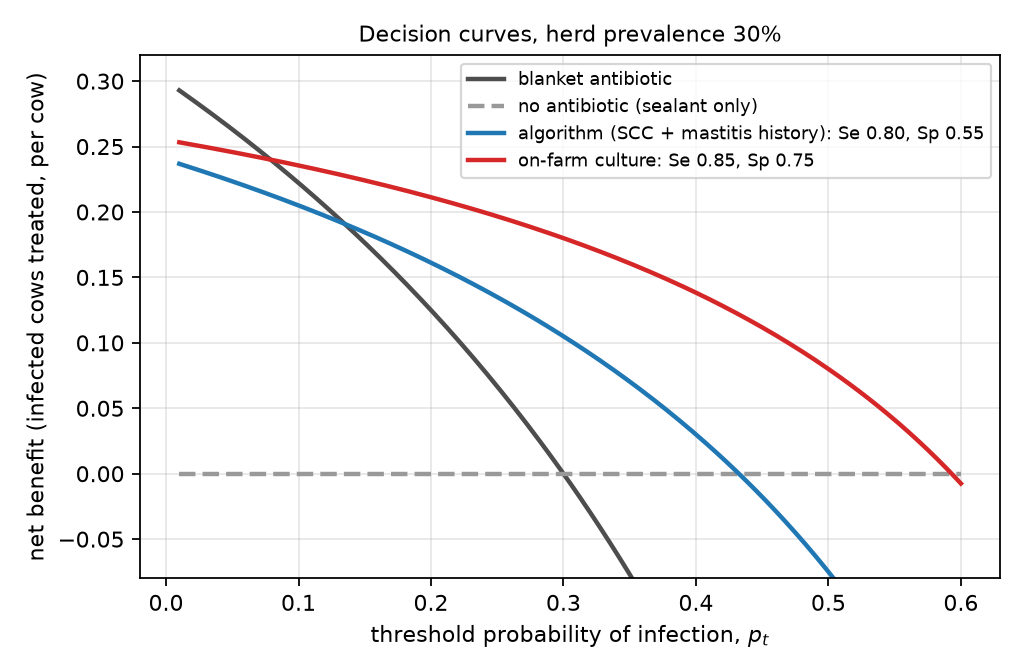
\includegraphics[width=0.72\linewidth]{fig_dca.png}
\caption{Decision curves for an illustrative herd with 30\% prevalence.}
\label{fig:dca}
\end{figure}
\begin{figure}[t]
\centering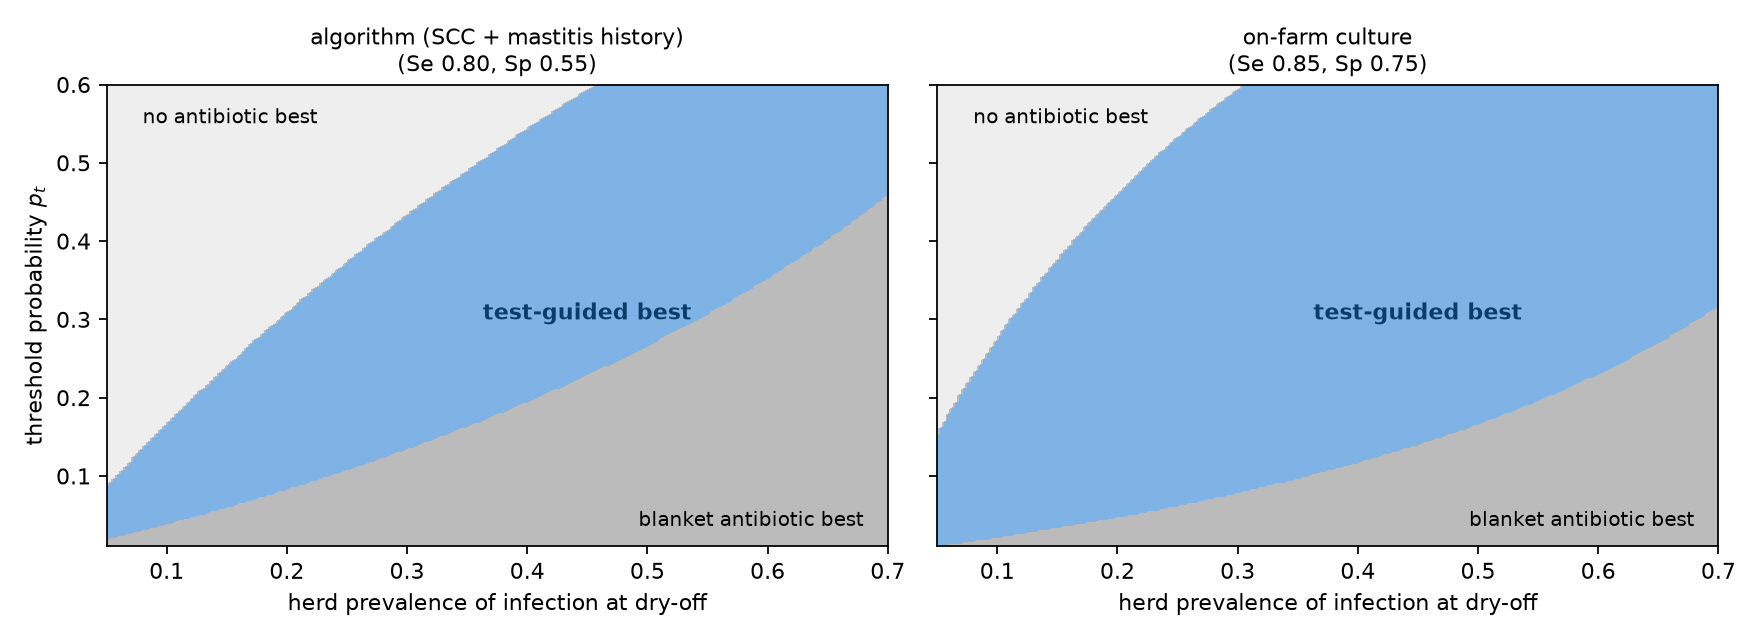
\includegraphics[width=\linewidth]{fig_regions.png}
\caption{Best strategy by herd prevalence and threshold probability.}
\label{fig:reg}
\end{figure}

\begin{table}[h]
\centering
\begin{tabular}{lccccc}
\toprule
herd prevalence & 10\% & 20\% & 30\% & 40\% & 50\% \\
\midrule
algorithm ($Se$ 0.80, $Sp$ 0.55) & 3.9--16.5 & 8.3--30.8 & 13.5--43.2 & 19.5--54.2 & 26.7--64.0 \\
culture ($Se$ 0.85, $Sp$ 0.75) & 2.2--27.4 & 4.8--45.9 & 7.9--59.3 & 11.8--69.4 & 16.7--77.3 \\
\bottomrule
\end{tabular}
\caption{Range of threshold probabilities $p_t$ (\%) for which the test-guided rule has the highest net benefit.}
\label{tab}
\end{table}

Figure~\ref{fig:dca} shows the decision curves at 30\% prevalence and Table~\ref{tab} the useful ranges.
\begin{itemize}
\item \textbf{Blanket therapy is best only for herds that care little about antibiotic use}, roughly $p_t$ below
8--14\% at 30\% prevalence. Stewardship-minded herds lie above this.
\item \textbf{No antibiotic at all} becomes best only at high thresholds (above 43\% for the algorithm, 59\% for
culture at 30\% prevalence): the sealant-only strategy is rarely optimal unless infections are rare.
\item \textbf{Culture dominates the algorithm} over the whole range shown, because it is more specific; the
algorithm's advantage is its zero marginal cost, which can be added to the harm term when needed.
\item \textbf{Prevalence moves the window.} In low-prevalence herds (10\%) the algorithm is useful only between 4\%
and 17\%; Figure~\ref{fig:reg} shows the full map.
\item \textbf{Under uncertainty} (Figure~\ref{fig:unc}), the culture-guided rule is best with probability above 0.8
for $p_t$ between 11.5\% and 47\%; the algorithm for $p_t$ between 19\% and 32\%.
\end{itemize}
\begin{figure}[t]
\centering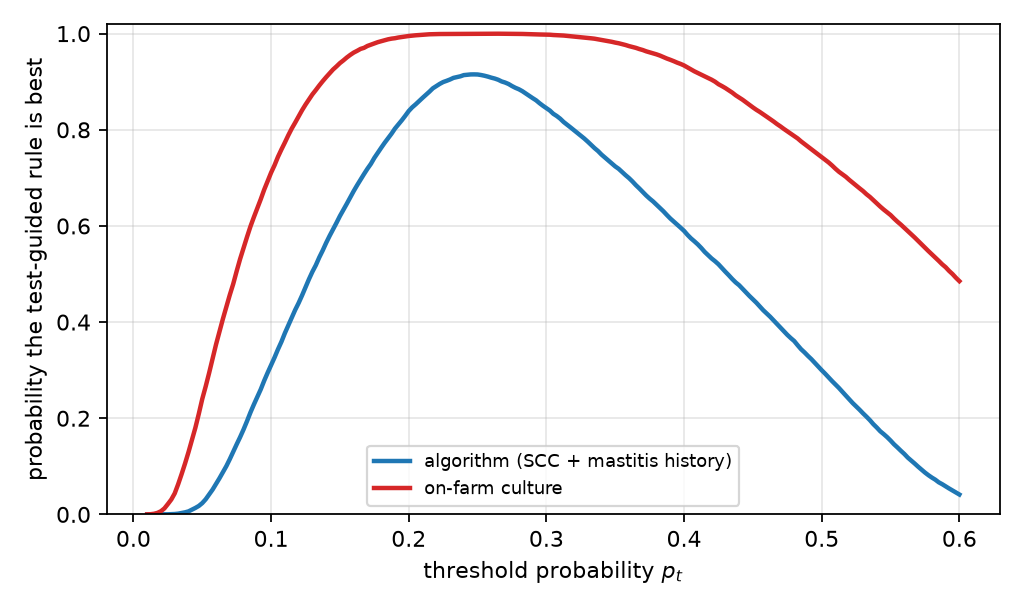
\includegraphics[width=0.72\linewidth]{fig_uncertainty.png}
\caption{Probability that the test-guided rule is best, under uncertainty in prevalence, sensitivity and specificity.}
\label{fig:unc}
\end{figure}

\section{Discussion}
DCA gives dairy veterinarians a decision tool that partial budgets do not: it places the stewardship trade-off in a
single, explicit number and shows, for a given herd, whether a test improves on treating all cows or none. The closed
form makes it usable without software. Two refinements are natural: a continuous risk score (for example from SCC
trajectories) evaluated by its own decision curve, and a test-cost term added to the harm side.

\paragraph{Limitations.} The parameter values are illustrative; cure and new-infection dynamics during the dry period
are summarised in the single benefit term; quarter-level decisions and herd-level costs are not modelled.

\paragraph{Reproducibility.} \texttt{experiment.py} regenerates every number and figure.

\paragraph{Origin of the question.} The question came from an automated forecast (Singularity v3, registered on 5
November 2026 with a SHA-256 fingerprint) that decision curve analysis would enter the subfield \emph{Animal Science
and Zoology}. The forecast concerned the arrival of the method, not the result of this note.

\begin{thebibliography}{9}
\bibitem{Vickers2006} A.~J.~Vickers, E.~B.~Elkin, Decision curve analysis: a novel method for evaluating prediction
models, \emph{Medical Decision Making} 26 (2006) 565--574.
\bibitem{Vickers2019} A.~J.~Vickers, B.~van Calster, E.~W.~Steyerberg, A simple, step-by-step guide to interpreting
decision curve analysis, \emph{Diagnostic and Prognostic Research} 3 (2019) 18.
\bibitem{Rowe2021} S.~M.~Rowe et al., Partial budget analysis of culture- and algorithm-guided selective dry cow
therapy, \emph{Journal of Dairy Science} (2021).
\end{thebibliography}
\end{document}
